\section{Management Component}

\subsection{Persisting messages in the DHT}

As already discussed, peers may go offline for longer time periods while the network is deployed.
When a peer is offline it misses all messages, once it is online again it would display outdated content until it receives new content. \footnote{Note that of course it is unavoidable that the content may become outdated while the peer is offline. However at least when it comes back online it should get the most recent state.}
Thus a solution is required for storing message for offline peers so that once online again they can retrieve the most recent message and update their displayed content.
We set the following requirements for our implementation:
\begin{itemize}
    \item Peers should be able to the retrieve the most recent content to display as soon as they join the network.
    \item Ability to scale with the number of peers so that ideally the burden for storing messages is spread evenly among the peers.
    \item Minimal storage and message overhead.
    \item Peers unexpectedly going offline should not result in message loss.
\end{itemize}
To solve this we implemented a Distributed Hash Table (DHT) that persists data in the network.

The prerequisite for our implementation is that shared state is maintained among all peers about which (authorized) peers are currently online. 
As already discussed in section \ref{p2p-network} a peer is never connected to all peers in the network, thus to get the full view of all online peers additional logic is required.
For this, peers exchange information about what peers they are connected to. 
Each time a peer established a connection to a new (authorized) peer, it informs the network of this event so that all other members can update their list of assumed online peers.
Analogously when a peer unexpectedly disconnects from another peer it also informs the network about it\footnote{It may happen that a connection closes but the peer is still in the network, therefore if a peer receives a \textit{DISCONNECTED} message about itself it directly sends a \textit{CONNECTED} with its own ID again.}.

This list serves as basis for mapping what peer stores what information.
To catch the case of nodes unexpectedly disconnecting messages are always stored by two other peers.
For each message that directed to a peer, the message is sent to that peer if it is online, and additionally to those two peers for storage.
The two peers are selected from the list of online peers by sorting the list by \textit{PeerId} and picking the next two peers after where the target's ID is / would be in the list.

% TODO: describe how re-publishing happens if peers join/ leave the network

\begin{figure}
    \centering
    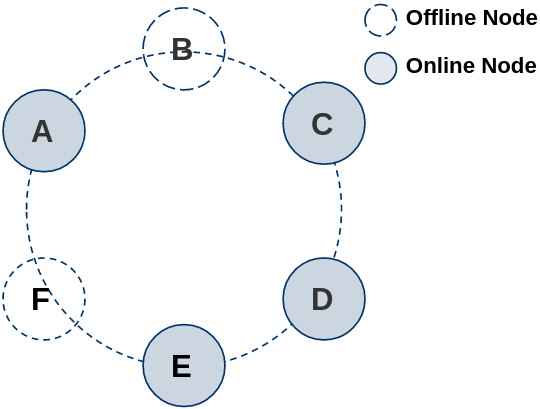
\includegraphics[width=0.3\textwidth]{assets/dht.png}
    \caption{DHT nodes arranged by ID in a circular list. The data for a node is persisted by the two subsequent online nodes. In this example the messages for A and B are both persisted by C and D}
    \label{fig:dht}
\end{figure}

